\documentclass{article}

% *****************************************************************
% Package things
% *****************************************************************
\usepackage[utf8]{inputenc}
\usepackage{mathtools}
\usepackage{amsmath}
\usepackage{amssymb}
\usepackage{enumitem}
\usepackage[hang,flushmargin]{footmisc}
\usepackage{booktabs}
\usepackage{color}
\usepackage{bbm}
\usepackage{footnote}
\usepackage{enumitem}
\usepackage{longtable}

\setlength\parindent{0pt}
\usepackage[anythingbreaks]{breakurl}

\usepackage{pgfplots}
\usepackage[margin=1in]{geometry}
\usepackage{hyperref}

\pgfplotsset{width=10cm,compat=1.9}


% *****************************************************************
% Estout related things
% *****************************************************************
\newcommand{\sym}[1]{\rlap{#1}}% Thanks to David Carlisle

\let\estinput=\input% define a new input command so that we can still flatten the document

\newcommand{\estwide}[3]{
		\vspace{.75ex}{
			\begin{tabular*}
			{\textwidth}{@{\hskip\tabcolsep\extracolsep\fill}l*{#2}{#3}}
			\toprule
			\estinput{#1}
			\bottomrule
			\addlinespace[.75ex]
			\end{tabular*}
			}
		}	

\newcommand{\estauto}[3]{
		\vspace{.75ex}{
			\begin{tabular}{l*{#2}{#3}}
			\toprule
			\estinput{#1}
			\bottomrule
			\addlinespace[.75ex]
			\end{tabular}
			}
		}

% Allow line breaks with \\ in specialcells
	\newcommand{\specialcell}[2][c]{%
	\begin{tabular}[#1]{@{}c@{}}#2\end{tabular}}

% *****************************************************************
% Custom subcaptions
% *****************************************************************
% Note/Source/Text after Tables
\newcommand{\figtext}[1]{
	\vspace{-1.9ex}
	\captionsetup{justification=justified,font=footnotesize}
	\caption*{\hspace{6pt}\hangindent=1.5em #1}
	}
\newcommand{\fignote}[1]{\figtext{\emph{Note:~}~#1}}

\newcommand{\figsource}[1]{\figtext{\emph{Source:~}~#1}}

% Add significance note with \starnote
\newcommand{\starnote}{\figtext{* p < 0.1, ** p < 0.05, *** p < 0.01. Standard errors in parentheses.}}

% *****************************************************************
% siunitx
% *****************************************************************
\usepackage{siunitx} % centering in tables
	\sisetup{
		detect-mode,
		tight-spacing		= true,
		group-digits		= false ,
		input-signs		= ,
		input-symbols		= ( ) [ ] - + *,
		input-open-uncertainty	= ,
		input-close-uncertainty	= ,
		table-align-text-post	= false
        }
% *****************************************************************
% Document starts here
% *****************************************************************

\begin{document}

\title{AK Replication a la Bayes}
\author{Rachel Anderson}

\maketitle

% Table 1
\begin{table}
\centering
\caption{OLS results using year/place of birth fixed effects and education dummies}
\estauto{ak_ols.tex}{1}{c}
\label{table1}
\end{table}

% Table 2
\begin{table}
\centering
\caption{IV resultst}
\estauto{iv.tex}{4}{c}
\label{table1}
\end{table}

%Table 3 -- will be first stage results 

\begin{figure}[h!]
\centering
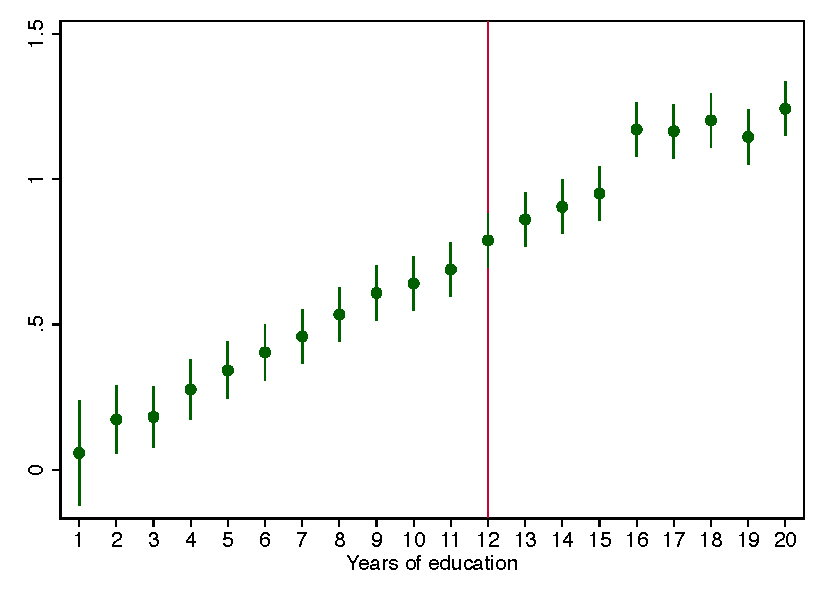
\includegraphics[width=0.7\textwidth]{../Figures/coefplot_ols.pdf}
\caption{Plot of OLS coefficients for education variables}
\end{figure}

\begin{figure}
\centering
  \begin{minipage}[b]{0.48\textwidth}
    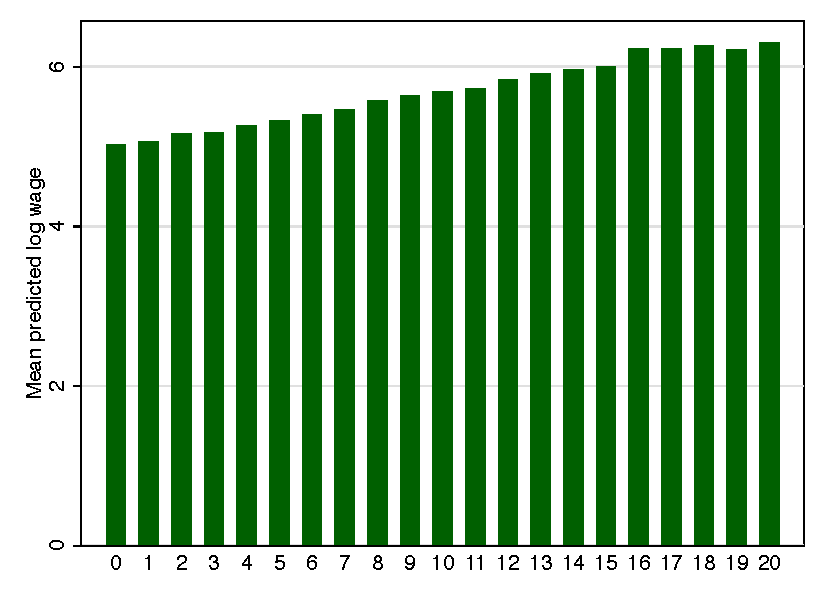
\includegraphics[width=\textwidth]{../Figures/logwage_ols.pdf}
    \caption{Predicted log-wage by education level}
    \label{fig:1}
  \end{minipage}
  \begin{minipage}[b]{0.48\textwidth}
    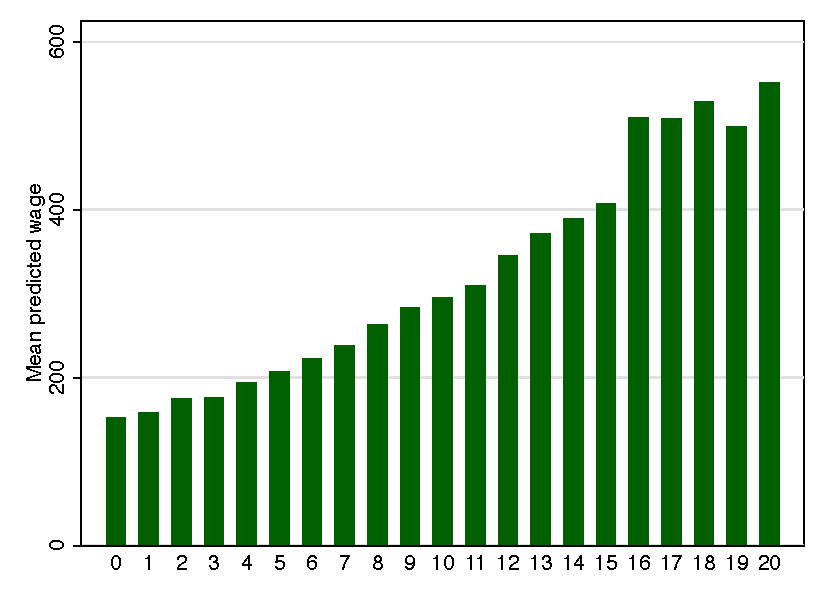
\includegraphics[width=\textwidth]{../Figures/wage_ols.pdf}
    \caption{Predicted wage by education level}
    \label{fig:2}
  \end{minipage}
\end{figure}

\section*{Bayesian Parts}

The model is 
\begin{gather}
\underset{n \times 1}{y} = \underset{n\times k}{X}\underset{k\times1}{\beta} + \underset{n\times1}{\epsilon} \\
\underset{n \times k}{X} = \underset{n\times L}{Z}\underset{L\times k}{\gamma} + \underset{n\times k}{\nu} \nonumber \\
\begin{pmatrix} \epsilon \\ \nu \end{pmatrix} \sim \mathcal{N}(0, \Sigma_1)\nonumber
\end{gather}

which implies

\begin{gather*}
y = \underset{n\times L}{Z}\underset{L\times k}{\gamma}\underset{k\times 1}{\beta} + \underset{n\times k}{\nu}\underset{k \times 1}{\beta} + \underset{n\times1}{\epsilon} \\
\begin{pmatrix} \nu\beta + \epsilon \\ \nu \end{pmatrix} \sim \mathcal{N}(0, \Sigma_2)
\end{gather*}

In the most simple case, with $k=1$ (one endogenous regressor), we can reparameterize the model:
\begin{gather}
\underset{n \times 2}{\mathcal{Y}} = \underset{n\times L}{Z}\underset{L \times 2}{\Pi} + \underset{n\times2}{\eta} \\
\iff \underset{n \times 2}{\begin{bmatrix} y \hspace{5pt}  x \end{bmatrix}} =  \underset{n\times L}{Z}\underset{L \times 2}{\begin{bmatrix}\gamma\beta \hspace{5pt} \gamma\end{bmatrix}} + \underset{n\times2}{\begin{bmatrix}\nu\beta + \epsilon \hspace{5pt} \nu\end{bmatrix}} \nonumber \\
\eta \sim \mathcal{N}(0, \Omega)
\end{gather}

If we impose the restriction that rank($\Pi$) = 1, the model in (2) traces out the same set of probability models for the data as in (1).  (This imposes that the elements of $\Pi$ are linear combinations of each other, since $\gamma\beta$ is a linear combination of $\gamma$ when ($L\geq k$).)

In the initial parameterization (Model 1), the likelihood is not integrable for a flat prior on $\beta$, and so it is useful to describe an uninformative prior over $\Pi$ in (2)\footnote{See the argument in Sims (2007)}.  In fact, a flat prior on $\Pi$ with no rank restrictions produces an integrable posterior if the sample size is not too small.  Hence, we can construct a ``flat" prior for (1) by transforming a flat prior over the reduced-rank submanifold of $\Pi$ into $(\beta, \gamma)$ space. The improper prior on $(\beta, \gamma)$ that emerges from this approach is (assuming $L=k=1$):
\begin{align*}
\left| \frac{\partial\Pi}{\partial(\beta, \gamma)} \left( \frac{\partial\Pi}{\partial(\beta, \gamma)} \right)'\right| ^{\frac{1}{2}} &= \left | \begin{bmatrix} \gamma & 0 \\ \beta & 1 \end{bmatrix}  \begin{bmatrix} \gamma' & \beta' \\ 0' & 1' \end{bmatrix}  \right | ^{\frac{1}{2}} \\
&= \begin{vmatrix}  \gamma\gamma' & \gamma\beta' + \gamma 1' \\ \beta\gamma' & \beta\beta' + 11'  \end{vmatrix} ^{\frac{1}{2}} \\
&= (\gamma\gamma')(\beta\beta' + 11') - (\gamma\beta'+\gamma1')(\beta\gamma') \\
&= || \gamma|| (1+\beta^2)^\frac{1}{2} 
\end{align*}

\section*{LIML}
Question 3 requires estimating model (2) with $k=1$, $L=3$ with LIML. The likelihood function of the data is:

\[
\ell (\beta, \gamma, \Omega) \propto \sum_{i=1}^{N} \left( - \frac{1}{2} \ln | \Omega | - \frac{1}{2} \begin{pmatrix} y_i - \beta x_i & x_i - Z_i\gamma\end{pmatrix} \Omega^{-1} \begin{pmatrix} y_i - \beta x_i  \\  x_i - Z_i \gamma\end{pmatrix} \right)
\]

Since $y_i, x_i$ are scalar, the likelihood can be written as:
\begin{gather*}
-\frac{N}{2}\ln | \Omega| - \frac{1}{2 | \Omega| }\sum_{i=1}^N \Big( (y_i - \beta x_i)^2\omega_{22} - 2(y_i - \beta x_i)(x_i - Z_i \gamma)\omega_{12} + (x_i - Z_i \gamma)^2\omega_{11}\Big) \\
-\frac{N}{2}\ln | \Omega| - \frac{1}{2 | \Omega| } \left(\omega_{22} \sum_{i=1}^N (y_i - \beta x_i)^2 - 2 \omega_{12} \sum_{i=1}^N (y_i - \beta x_i)(x_i - Z_i \gamma) + \omega_{11} \sum_{i=1}^N (x_i - Z_i \gamma)^2 \right)
    \end{gather*}
    
where $\Omega = \begin{pmatrix} \omega_{11} & \omega_{12} \\ \omega_{12} & \omega_{22} \end{pmatrix}$.  
\\

In higher dimensions, this inner part corresponds with the cross product/second moment of the data, so that we can optimize code by passing the second moment as an argument.  
\\

Take the singular value decomposition of $\gamma$:
\[ \gamma = U S V' \]
where $U$ and $V$ 

The likelihood is combined with an improper flat prior:
\[
\pi(\beta, \gamma) \propto \sum_{i=1}^{k} \log(\text{diag}(d)) \equiv f(\gamma)
\]
where $d$ is defined according to the singular value decomposition of $\gamma = u d v'$.  When $L =1$, as in part 3, this is equal to $||\gamma ||$ same as we derived in the section above. 

\end{document}